
\chapter{Risultati}
\label{risultati}

\section{Metriche di valutazione}
Le metriche di valutazione utilizzate per testare la qualità dei modelli sono state:
\begin{itemize}
\item \textbf{Precision}: il rapporto $\frac{t_p}{t_p+f_p}$ dove $t_p$ è il numero di veri positivi e $f_p$ il numero di falsi positivi. Intuitivamente è l'abilità del classificatore di non marcare come positivo un campione negativo.
\item \textbf{Recall}: il rapporto $\frac{t_p}{t_p+f_n}$  dove $f_n$ sono i falsi negativi. Intuitivamente è l'abilità del classificatore di trovare tutti i campioni positivi.
\item \textbf{F-score}: è definito come la media armonica tra \textit{precision} e \textit{recall}: 
\[F_1 = 2 \cdot \frac{1}{\tfrac{1}{\mathrm{recall}} + \tfrac{1}{\mathrm{precision}}} = 2 \cdot \frac{\mathrm{precision} \cdot \mathrm{recall}}{\mathrm{precision} + \mathrm{recall}}\]
\item \textbf{Area sottesa da Receiver Operating Characteristic}:  metodo grafico per la valutazione della qualità di un classificatore binario al variare della soglia di discriminazione. E' creata graficando la frazione dei veri positivi rispetto ai campioni positivi ($tpr$ = True positive rate) contro la frazione dei falsi positivi rispetto ai campioni negativi ($fpr$ = False positive rate). L'area sottesa dalla curva ROC equivale alla probabilità che il classificatore predica un campione positivo casuale rispetto ad un campione negativo casuale. Formalmente è definita da:
\[ A = \int_{\infty}^{-\infty} \mbox{TPR}(T) \left(-\mbox{FPR}'(T)\right) \, dT = \int_{-\infty}^{\infty} \int_{-\infty}^{\infty} I(T'>T)f_1(T') f_0(T) \, dT' \, dT = P(X_1 > X_0)\]
dove 
$X_{1}$ è il punteggio per un'istanza positiva e $X_{0}$ è il punteggio per un'istanza negativa, mentre $f_{0}$ e $f_{1}$ sono densità di probabilità che un campione sia negativo ($1$) o positivo ($0$)
\end{itemize}

\section{Classificatore Random Forest}
Il classificatore Random Forest è stato testato in diverse configurazioni. La configurazione che è stata presentata nella sezione \ref{imp:randomforest} ha mostrato i migliori risultati in ogni test.

Il classificatore è stato testato dapprima testato con le seguenti famiglie di malware, contro un subset di dimensione simile di domini provenienti dalla classifica Alexa.

\begin{table}[!ht]
    \centering
    \begin{tabular}[t]{l}
    \toprule
    Malware Families \\
    \midrule
legit \\
cryptolocker \\
zeus \\
pushdo \\
rovnix \\
tinba \\
conficker \\
matsnu \\
ramdo \\
\bottomrule
\end{tabular}
\caption{\label{tab:malware}}
\end{table}

Il dataset così riunito è stato separato in due parti disuguali: il 90\% è stato utilizzato come dataset di training mentre il restante 10\% come testing in maniera da evitare il fenomeno di overfitting. I risultati della predizione sul dataset di testing sono mostrati di seguito in figura \ref{fig:repdga} e figura \ref{fig:rocdga}. A fianco dell'etichette \textit{legit} e \textit{DGA} è indicato il numero di campioni utilizzati per le due categorie. Come si può notare la performance del classificatore

\begin{figure}[!htbp]
    \centering
    \includegraphics[width=\columnwidth]{figures/rndf_tra_nosup_nosup/class_rep.png}
    \caption{Report di classificazione su un subset di domini reali (legit) e malevoli (DGA).\label{fig:repdga}}

    \centering
    \includegraphics[width=\columnwidth]{figures/rndf_tra_nosup_nosup/roc_plot.png}
    \caption{Area sottesa dalla curva ROC per il test con domini di tabella \ref{tab:malware}.\label{fig:rocdga}}
\end{figure}

Lo stesso classificatore è stato testato inserendo \textit{suppobox} all'interno delle famiglie DGA. Si è scelto tale malware come campione esterno in quanto presentava la maggiore differenza rispetto alle famiglie mostrate in tabella \ref{tab:malware}. Non è stato fatto un ulteriore training con suppobox. I risultati si possono vedere in figura \ref{fig:repsup} e \ref{fig:rocsup}. Come si può notare la performance ne è pesantemente influenzata, introducendo una grande percentuale di falsi nelle predizioni effettuate dal classificatore.

\begin{figure}[!htbp]
    \centering
    \includegraphics[width=\columnwidth]{figures/rndf_tra_nosup_sup/class_rep.png}
    \caption{Report di classificazione su un subset di domini reali (legit) e malware, comprendenti suppobox (DGA).\label{fig:repsup}}

    \centering
    \includegraphics[width=\columnwidth]{figures/rndf_tra_nosup_sup/roc_plot.png}
    \caption{Area sottesa dalla curva ROC per il test con  suppobox.\label{fig:rocsup}}
\end{figure}

Come ultimo test è stato eseguito il training aggiungendo al precedente dataset di training una parte di domini generati da suppobox (Figura \ref{fig:repall} e \ref{fig:rocall}). Come si può notare la performance è migliorata sensibilmente, non raggiungendo comunque i risultati eccellenti del primo test.

\begin{figure}[!htbp]
    \centering
    \includegraphics[width=\columnwidth]{figures/rndf_tra_sup_sup/class_rep.png}
    \caption{Report di classificazione su un subset di domini reali (legit) e malware, comprendenti suppobox (DGA).\label{fig:repall}}

    \centering
    \includegraphics[width=\columnwidth]{figures/rndf_tra_sup_sup/roc_plot.png}
    \caption{Area sottesa dalla curva ROC per il test con domini reali e malware (comprendenti suppobox).\label{fig:rocall}}
\end{figure}

\section{Classificatore Neurale}

\section{Autoencoder}

\section{Generative Adversarial Network}
